\chapter{X-ray Observatories and their Source Catalogs}
\label{chap2}

As mentioned, observing AGN that have experienced dramatic and long-term variability in their X-ray emission is rare.
By increasing the time between successive observations for all objects, we can increase the detection rates, suggesting that we use data from instruments that observed at mutually exclusive time frames.
This can be achieved by using data obtained with the Einstein Observatory and the Chandra X-ray Observatory. 
For reasons that will become apparent in Chapter 3, we also use the R\"{o}ntgen Satellite (ROSAT), a mission that operated in between Einstein and Chandra. 
The following sections will discuss the specifications of each of the observatories and the serendipitous source catalogs complied from the observations conducted with them.


\section{The Einstein X-ray Observatory}
\label{sub2_1}

The Einstein Observatory (shown in Fig. 2.1) launched on November 13, 1978 and was in operation until April 1981 (2 years 5 months). 
It was the second observatory launched as part of NASA’s High Energy Astrophysics Observatory (HEAO) program.
Thus, Einstein is also known as HEAO 2 (or HEAO B). 
The Einstein mission was particularly important because it was the first imaging X-ray telescope placed into orbit.

\begin{figure}[H]
\centering
\scalebox{0.8}{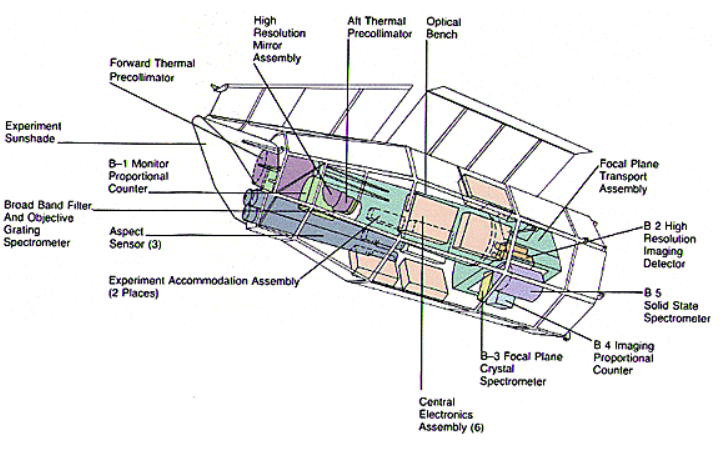
\includegraphics[scale=1]{images/einstein.png}}
\caption{Schematic of the Einstein Observatory from \cite{giacconietal1979}. }
\label{imbeded_fb}
\end{figure}


\subsection{Einstein's Design}

The telescope’s design was a Wolter type I design, which used a parabolic primary mirror followed by a hyperbolic secondary. 
The geometry of such a design (shown in Fig. 2.2) uses grazing incidence optics to reflect X-ray photons at very shallow angles towards one focal point. 
The grazing angle required to successfully reflect X-rays in 0.2-4 keV band was about 1$^{\circ}$.
By nesting several mirror shells with the same focal plane, the collecting area was increased without causng much loss in resolution.
Therefore, the Einstein telescope consisted of 4 nested reflecting surfaces with the innermost and outermost surfaces having a diameter of 33cm and 56cm, respectively.
This mirror design resulted in an effective area of 400 cm$^2$ at 0.25 keV and 30 cm$^2$ at 4 keV. 
It provided an angular resolution of 5’’ on axis but 1.5’ at the edge of the 1 degree field of view \citep{giacconietal1979}.

\begin{figure}[H]
\centering
\scalebox{0.8}{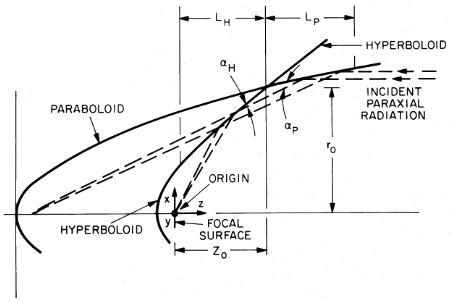
\includegraphics[scale=1]{images/einstein_wolter_type_one_design.png}}
\caption{The geometry of the Wolter type I X-ray telescope design from  \cite{giacconietal1979}. }
\label{imbeded_fb}
\end{figure}


\subsection{Einstein's Instruments}


 In the telescope, there were four main instruments that it carried: the Imaging Proportional Counter (IPC), High Resolution Imager (HRI), the Solid State Spectrometer (SSS), and the Focal Plane Crystal Spectrometer (FPCS). 
 Of the four, the IPC was the most widely used. 
 The IPC was a gas-filled detected that contained electrodes arranged with an anode in between two cathodes. 
 The anode is accelerated by X-ray photons. 
 It then discharges and sends an induced signal to the cathodes. 
 This allowed the IPC to determine the position of an event to 1 arcmin accuracy over a 60 x 60 arcmin FOV. 
 However, the centroid of the point source was determined to greater precision than 1 arcmin. 
 The IPC had a field of view of 75’ x 75’ but had less position precision 1 arcmin at the periphery of this field of view.
 It has a angular resolution of 1’, an effective area of 100 cm$^2$ at $\sim 1$ keV, and operated in the 0.15-4 keV energy range \citep{giacconietal1979}.


 
 \subsection{X-Ray Surveys with Einstein}



One of Einstein’s most notable scientific achievements was the detection of thousands of serendipitous sources.
That is, in observations of a target object, objects in the periphery are also detected due to its large field of view.
A fairly large portion of the sky was in each IPC observation, which made partial sky surveys possible.
Due to the nature of the serendipitous sources, these catalogs are dependent on how the data is interpreted and processed.
Different biases and source detection methods can lead to different sources being considered real or spurious.

The Medium Sensitivity Survey (MSS; Gioia et al. 1986) used the IPC to create a sample of 680 sources at high latitude sky using 1160 IPC images. 
This totaled a sky coverage of 590 deg$^2$.
The sensitivity of the MSS ranged from $5\times 10^{-14}$ to $3\times 10^{-12}$ erg cm$^{-2}$ s$^{-1}$ in the 0.3 - 3.5 keV energy band.
The selection process of the MSS also considered only the inner $60' \times 60'$ field of view of an image and considered sources with a signal-to-noise ratio (SNR) greater than a 5$\sigma$ threshold.
It also omitted IPC fields that were within 20 deg of the Galactic plane in order to safely assume a neutral hydrogen column density of $3\times 10^{20}$ cm$^{-2}$. 
Ultimately, the MSS was used to construct an X-ray selected quasar sample.

The efforts of the MSS were later expanded in the Einstein Extended Medium Sensitivity Survey (EMSS; Gioia et al. 1990).
The EMSS had a primary goal of detecting different populations of discrete sources responsible for the X-ray background.
Like the MSS, the EMSS included sources to the same sensitivity range and also enforced the same position restriction ($|\text{b}| >$ 20 deg). 
The EMSS, however, re-analyzed all the IPC image fields to exclude only fields that were centered on bright sources and/or extended sources.
It also excluded fields containing groups or association of objects. 
The EMSS lowered their SNR threshold to 4$\sigma$.  
As a result, the  EMSS contained 835 sources from 1435 images  from the improved calibration techniques which gave a total sky coverage of 778 sq degrees of high latitude sky  \citep{gioia1990}.

In order to incorporate the faintest sources from Einstein (and fainter sources that those found in EMSS) \cite{moran1996} constructed a new catalog using Einstein’s IPC field images which included sources exceeding an SNR threshold of 2$\sigma$.
Consequently, the catalog is named the Einstein Two-Sigma Catalog (ETS).
The primary goal of the ETS was to obtain a more complete picture of the components of the cosmic X-ray background.
In order to do this, different criteria were employed to select IPC fields.
First, the ETS excluded all images centered on sources of bright, diffuse emission as these are objects likely to contain a high concentration of spurious 2$\sigma$ sources.
Sources within 10 degrees of the Galactic plane were excluded with careful omission of galactic supernova remnants and fields within the Magellanic clouds.
Under these criteria, 2520 IPC images were used to construct the catalog (as opposed to 1435 images used in the EMSS). 
The IPC images (aside from the 4’ strips that lie on top of the window support ribs) used the entire 75’ x 75’ FOV of the image rather than the 60’ x 60’ FOV that MSS and the EMSS considered.
The catalog includes the target/center source as well as the sources in the periphery of each field. 
This results in a sky coverage of 1850 deg$^2$, 2.3 times that of the EMSS. 
The mean exposure times for the images was 3900 seconds while the median was 2200 seconds \citep{moran1996} .

To search for the sources in the images, \cite{moran1996} used an algorithm similar to that described in \cite{hamilton1991}. 
Using their algorithm directly resulted in uncertainties in source validity below 3.5$\sigma$.
Thus, modifications to their source-search algorithm were made. 
The source search began with the construction of two maps (one for the exposure time and another for the counts) of the IPC observations. 
Flat fielding is applied to the exposure map to account for the vignetting and gain variations in the detector wires.
The maps are combined and then a signal to noise ratio is computed for a putative source centered on each pixel.
Starting with a detection threshold of 10$\sigma$ and iteratively reducing the threshold to 2$\sigma$, any pixel that exceeds the threshold is considered a source and is then omitted in order to avoid contaminating the remaining iterations.
At lower SNR thresholds, the background annulus is increased since the minimum area used to compute the background noise becomes stricter. 
This increases the validity of the detected sources at these thresholds as it reduces the number of false sources.
Initially, 49,537 sources are detected in all of the IPC field images considered. 
After omitting the duplicates (keeping the detection with the highest SNR), 46,186 sources complete the ETS. 
Of these, 4,764 have a SNR of 3.5$\sigma$ or higher. From the soft X-ray log N($>$S) - log S relation modeling, it was determined that 28\% ( about 13,000) sources from the full ETS are real.
Below 4$\sigma$, the percentage is 22\% \citep{moran1996}. 
Thus, the ETS provides the highest number of real sources compared to the MSS and EMSS.
Figure 2.3 sows the source locations of the ETS catalog.


\begin{figure}[t]
\centering
\scalebox{0.22}{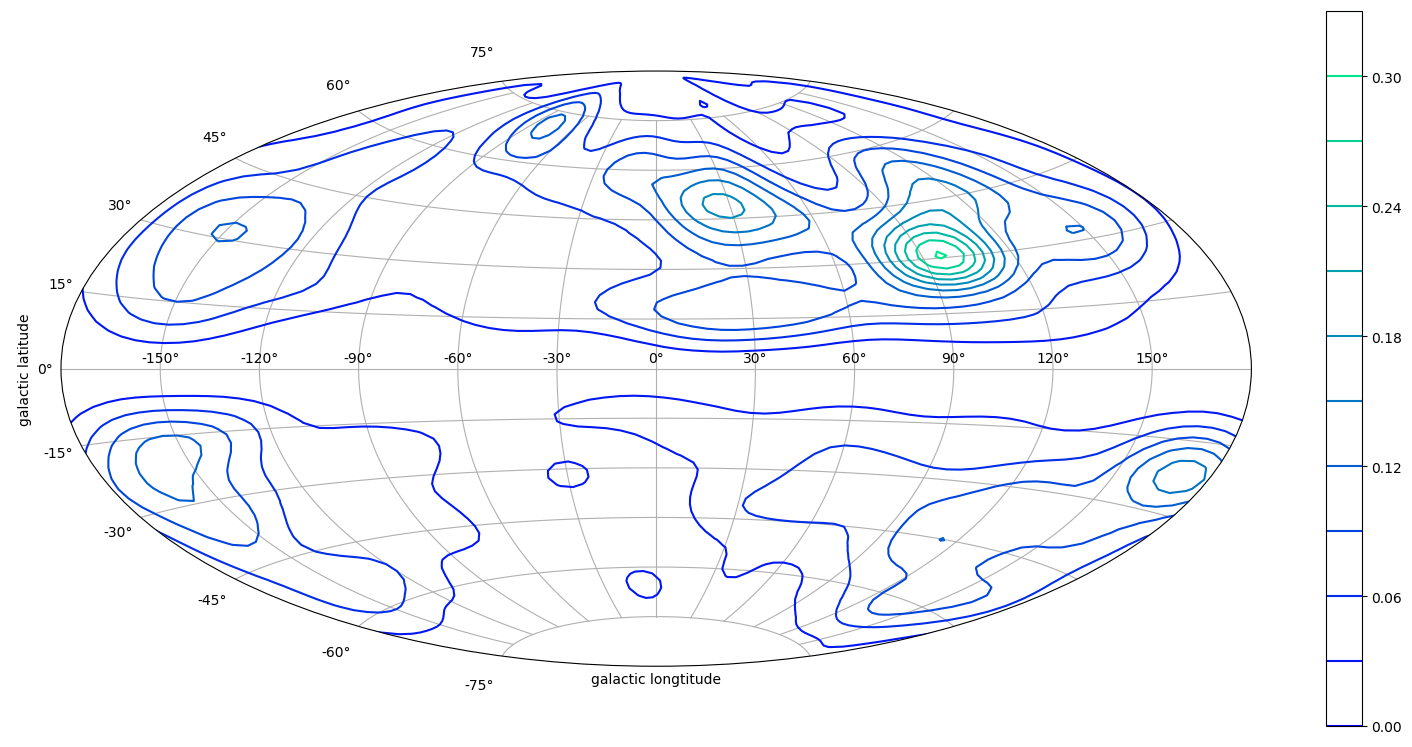
\includegraphics[scale=1]{images/ets_exp_map_contour_lines.png}}
\caption{The location of all sources from the Einstein Two-Sigma Catalog. }
\label{imbeded_fb}
\end{figure}

\FloatBarrier

\subsection{Optical Follow up of the IPC Sources}


Since the construction of the various X-ray catalogs using the IPC, optical follow ups have spectroscopically classified many of them. 
In the EMSS, the optical identification procedure involved identifying the object class based on optical spectroscopy and using the IPC X-ray flux and photometric magnitudes to compute X-ray-to-optical flux ratios, which also allows for object classification.
From this, 96\% percent of the 835 sources in the EMSS were identified. 
Of those identified, AGN made up the majority with 51.1\%. 
Galactic stars were next with 25.8\% of the catalog \citep{stocke1991}.

In the ETS, sources were optically identified by cross-correlating the data with the Green Bank 6cm and Texas 80 cm radio catalogs (where a large portion of the sources in these two radio catalogs had counterparts in VLA observations).
Allowing a separation limit of 60’’, the ETS matched to 598 6cm radio sources with a 87\% likelihood and it matched to 589 80cm radio sources with a 85\% likelihood. 
Optical spectroscopy was conducted on a few (40) of the radio-matched Einstein sources in three observing runs.
From this, the radio-selected X-ray sources was found to be mainly composed of quasars (17), with 3 of them being high redshift quasars.
At the time, one of the sources in the sample, 1508+5714, was the second most distant X-ray source known at a redshift of z = 4.30.
Other sources in the sample included ellipticals, narrow-line and broad-line galaxies, Seyferts, and liner galaxies \citep{moran1996}.

\cite{moran1996} additionally matched the ETS to the IRAS Faint Source Catalog to investigate the contribution of star forming galaxies, known to be bright infrared sources, have on the cosmic X-ray background. 
Spectra were obtained for the sample of bright infrared and X-ray sources that were a result of the cross correlation.
From spectroscopic identification of this sample, broad line AGN were found to be the dominant class.
\cite{moran1996}'s sample also found 15 new narrow-line Seyfert 1 galaxies, which characteristically have a full-width half-maximum value of H$\beta$ less than 2,000 km s$^{-1}$, a strong OIII line compared to the H$\beta$ line, and narrow FeII emission lines.
With a total of narrow-line Seyfert 1s appearing in the sample, their abundance was unexpected, but because of their known bright infrared properties, their inclusion was not.
A significant presence of star forming was not found in the sample, so evidence of them contributing to the cosmic X-ray background remained small \citep{moran1996}.



\section{The R\"{o}ntgen Satellite (ROSAT)}
\label{2_2}

The R\"{o}ntgen satellite (ROSAT;  See Fig. 2.4) was a German X-ray observatory designed at the Max-Planck Institute to carry the first all-sky suvey with an imaging X-ray telescope. 
ROSAT launched on June 1, 1990 and operated for 8 years and 8 months until its eventual demise in February 1999. 
During its mission, it was operated from the German Space Operations Center in Oberpfaffenhofen, Germany. 
ROSAT had an All-Sky Survey at the start of its mission and after, it continued through pointed observations \citep{Truemper1982}.



\begin{figure}[H]
\centering
\scalebox{0.7}{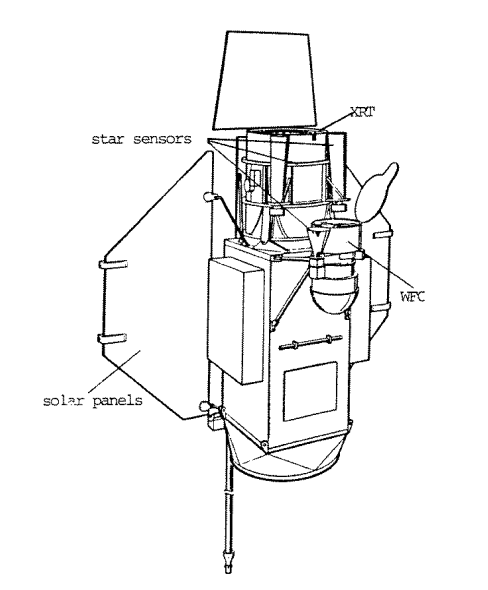
\includegraphics[scale=1]{images/rosat.png}}
\caption{Schematic of the ROSAT from \cite{Briel1996}. }
\label{imbeded_fb}
\end{figure}

\subsection{ROSAT's Design}

ROSAT was composed of two primary components: the X-ray Telescope and the Wide Field Camera. The X-ray Telescope had grazing incidence Wolter type-1 design. 
It consisted of 4 nested Wolter type-1 mirror shells.
The mirrors consisted of a zerodur substrate coated with a thin layer of gold.
The zerodur is a glass with a negligible coefficient thermal expansion and the gold coating allowed for improved X-ray reflection. at soft X-ray energies.
The optics design afforded a maximum aperture of 83.5cm and a focal length of 240cm. 
The average grazing angles for reflection occured between 1$^{\circ}$ and 2$^{\circ}$,depending on the subshell \citep{Briel1996}.

The Wide Field Camera has 3 nested mirrors (seperate from the XRT’s mirrors) in a Wolter-Schwarzchild design. 
They were made with aluminium and also coated with a thin layer of gold and had an average grazing angle of 7.5$^{\circ}$.
It provided a collecting area of 456 cm$^2$ at 1 keV. 
This assembly had a focal length of 0.525 meters. 
The instruments at the focal plane consisted of a curved microchannel plate and a carousel with 8 filters. 
The Wide Field Camera had a 5$^{\circ}$ field of view with a spatial resolution of 2.3'.


\subsection{The XRT's Instruments}

The X-ray Telescope had two imaging instruments at its focal plane: the Position Sensitive Proportional Center (PSPC) and the High Resolution Imager (HRI). 
Of the two, the PSPC was more widely used. It consisted of four componentes: PSPC-A, PSPC-B, PSPC-C, and PSPC-D, each 8cm $\times$ 8cm in size \citep{Truemper1982}. The PSPC-A and PSPC-D were only used for ground calibrations and were spares during ROSAT's mission.
They are all multiwire proportional counters where each electrode (anode and cathode) is a wire grid. 
The grids were inside of a counter filled with gas which had the following mixture: 65\% argon, 20\% xenon, and 15\% methane.
PSPC-C was meant to be the primary detector for ROSAT’s mission (and operated as such for most of ROSAT’s All Sky Survey) until the telescope scanned the sun, which destroyed the detector. 
Afterwards, the PSPC-B carried on with the mission and was used for all of the pointed observations. 
The PSPC had a 2$^{\circ}$ diameter field of view,  a spatial resolution of 0.25’ at 1 keV, and an effective area of 240 cm$^2$ at 1 keV. 
It operated in the 0.1 - 2.4 keV band.
The PSPC provided higher sensitivity, better spatial resolution, and lower background noise (from instrument and sky) than Einstein \citep{Belloni1994} .

\subsection{The ROSAT All-Sky Survey}


As mentioned earlier, ROSAT was launched with the intent of carrying out the first imaging all sky survey in the soft X-ray band (0.1-2.4 keV). 
The ROSAT All-Sky Survey (RASS) was a six month mission from July 1990 (a few weeks after its launch) until January 1991. 
During this survey period, the sky was scanned in great circles of 2$^{\circ}$ strips which intersected at the ecliptic poles. 
The total exposure time of the survey was 1.031 x 10$^7$ seconds (119.36 days) but the exposure time varied widely by region in the sky (see Fig 2.5 showing the exposure map of the RASS). 
Because of the way the RASS scanned the sky, the ecliptic equator averaged 400 seconds of exposure time while the ecliptic poles had a maximum exposure of 40,000 seconds \citep{voges1992}.




\begin{figure}[H]
\centering
\scalebox{0.8}{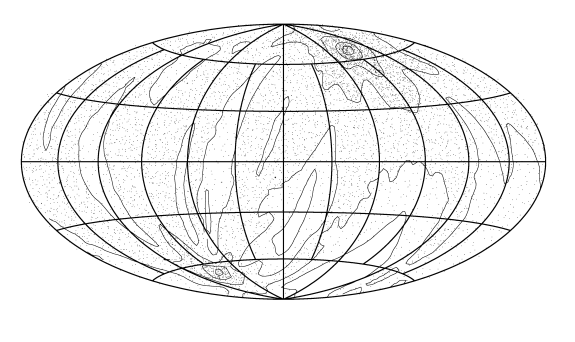
\includegraphics[scale=1]{images/rosat_all_sky_survey_exp_map.png}}
\caption{The logarithmic exposure map of the ROSAT's all sky survey where the longer exposures are darker. This projection shows the vernal equinox at the center and has right ascension (RA) increasing to the left. From \cite{Briel1996}. }
\label{imbeded_fb}
\end{figure}

The completion of the RASS mission produced a large amount of data for processing. 
\cite{voges1999} used these data to construct the ROSAT All-Sky Survey Bright Source Catalog (RASS-BSC) which picked out the brightest and most robustly detected sources from the RASS. 
To make the catalog, the 2$^{\circ}$ strips were analyzed using two source detection algorithms: a sliding window technique and a maximum-likelihood method. 

For each strip, a $3 \times 3$ pixel window moves across the photon image. 
At each of these steps, the photon count is added and compared to the background which is taken to be the 16 pixels surrounding the window. 
For extended sources, the window is increased but the background-to-source ratio of 16:9 is preserved. 
Using the sources produced from this method, circular regions with a radius equal to the window size are cut out. 
Another sliding window technique is performed and the two source lists created are merged and used as the input for the maximum likelihood method.
This method now considers each photon separately to allow for proper calibration with respect to the point spread function, which varies drastically with the off-axis angle.
The method outputs a source position and an existence likelihood. 
Finally, \cite{voges1999} selected the sources that have an existence likelihood of $\geq$ 15, at least 15 source photons, and a source count rate in the 0.1 - 2.4 keV energy band is $\geq$ 0.05 counts per second. 
After an additional screening process, the RASS-BSC had 18,8111 sources.
A similar procedure was done to generate the ROSAT All Sky Survey Faint Source Catalog (RASS-FSC; existence likelihood $\geq$ 6.5) which had 105,924 sources \citep{voges2000}.
Combining the two source catalogs produced the ROSAT 1RXS catalog.

A second, more recent ROSAT all-sky survey source catalog, called the 2RXS catalog, was constructed and released by \cite{boller2016}. 
Overall, The 2RXS catalog used similar procedures but made various improvements to them.
One of the main improvements in the 2RXS’s detection technique was that rather than using the $6.4^{\circ} \times 6.4^{\circ}$ images, it used smaller, $2.27^{\circ} \times 2.27^{\circ}$ images. 
This allowed for better determination of the local background. 
As a result, detection likelihood values are calculated with greater precision. 
Using this new improved detection method, \cite{boller2016} found that 12,000 sources in the RASS-FSC have a much lower likelihood value than originally calculated, which led them to be omitted from 2RXS. 
In total, the 2RXS has 129,192 sources (22,228 of them considered bright sources using the same criteria as the 1RXS). 
The distribution of likelihood values ranged from 6.5 to 26,198 and played a key part in the number of spurious sources. 
At a likelihood threshold of 6.5, there was a spurious detection rate of 37\%. 
Increasing the maximum likelihood threshold to 9 yields a catalog of 71,000 sources with a spurious detection rate of 5\%.
At a likelihood value of 11.01, only 1\% of the sources will be spurious. 
The exposure times of the full 2RXS catalog ranged from 7 seconds to 39,214 seconds. 
In total, the 2RXS covers 97\% of the sky with exposure time greater than 100 seconds. 

\subsection{Optical Follow Up to RASS Sources}

Once the 1RXS and 2RXS were completed, the natural progression was to optically identify the X-ray sources.
\cite{boller1992} used a subset of 14,708 extragalactic IRAS sources from the Point Source Catalog to cross correlate with the 1RXS. 
The IRAS subset was selected such that there is a strong likelihood that the source has an optical counterpart in the NASA/IPAC Extragalactic Database (NED).
Cross matching the IRAS sources and the 1RXS resulted in 244 IRAS galaxies with an X-ray counterpart from the 1RXS. 
Of these, 222 of them had optical counterparts identified by NED. 
104 of them additionally had redshifts, which allowed for the calculation of their X-ray luminosity.
The breakdown of these optically identified sources with an X-ray luminosity measurement were as follows: 50\% Seyferts, 44\% Spirals, 3\% Ellipticals, and 3\% quasars \citep{boller1992}.

In an effort to understand the role that luminous infrared sources like star-forming galaxies play in the cosmic X-ray background, \cite{moran1996} set out to obtain spectroscopic classification of the IRAS sources detected in the ROSAT All Sky Survey from \cite{boller1992}.
This was done by combining new optical spectroscopy with a thorough literature review. 
As a result of this, 210 of the sources from \cite{boller1992} were classified using new optical spectra. 
The majority of these sources turn out to be broad emission-line AGN. 
Thus, \cite{moran1996} find little evidence that starburst galaxies make up a significant portion of the X-ray background. 
In the process of classifying all of the sources, a new class of starburst/Seyfert composite galaxies was discovered. 
That is, while the optical spectra is dominated by features typical of starburst galaxies, they have X-ray luminosities typical of Seyfert galaxies. 
It is reasoned that these sources are Seyfert galaxies where their AGN component is obscured.

Additional efforts to optically identify sources in the RASS catalog include the Hamburg/RASS Catalog (HRC) by \cite{zickgraf2003} and those by \cite{gioia2003} for sources in the NEP.
The HRC was constructed by matching a patch of sky from the RASS-BSC ($\left|\text{b}\right| \geq$ 30$^{\circ}$ and dec $\geq$ 0$^{\circ}$) totaling 5341 X-ray sources with the Hamburg Quasar Survey.
This resulted in 82\% of 5341 sources being identified. AGN made up the large majority of the X-ray sources (42\%) followed by sources with stellar counterparts, which represented 32\% \citep{zickgraf2003}. 


\cite{gioia2003} focused on optically identifying sources in the NEP.
This was done in an extensive program that lasted 9 years (1991 - 2000) to observe the 445 sources from RASS in the NEP. 
Most of the observing was done at Mauna Kea (100 nights of observing) with a few observations at the University of Hawaii’s 2.2m telescope, the Canada-France-Hawaii 3.6m telescope and the Keck 10m telescope. 
In the end, after obtaining all the spectra needed, \cite{gioia2003} were able to identify 99.6\% of the sources and determine redshifts for the extragalactic ones.
The breakdown of classifications is similar to the results of \cite{zickgraf2003}.  
\cite{gioia2003} found 49\% of sources to be AGN (both type 1 and type 2) followed by 34\% of sources which had stellar counterparts. 
Clusters and groups of galaxies made up 1\% of the sources observed \citep{gioia2003}.




\section{The Chandra X-ray Observatory}
\label{2_3}


Originally called the Advanced X-Ray Astrophysics Facility when proposed by R. Giaconni, the Chandra X-ray observatory (shown Fig. 2.6) is one of NASA’s Great Observatories alongside the Hubble Space Telescope, the Compton Gamma Ray Observatory and the Spitzer Space telescope. 
Chandra launched on July 23, 1999 in the Space Shuttle Columbia with an initial planned mission of five years. 
At the time of this writing, Chandra’s mission is still ongoing, having a mission life of more than 20 years now.


\begin{figure}[H]
\centering
\scalebox{0.55}{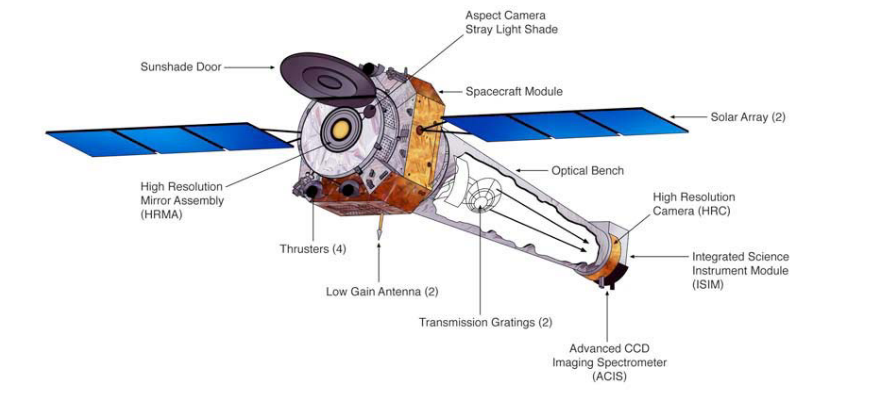
\includegraphics[scale=1]{images/chandra.png}}
\caption{Schematic of the Chandra X-ray Observatory from \cite{weisskopf1999}. }
\label{imbeded_fb}
\end{figure}

\subsection{Chandra's Design}

The Chandra X-ray Observatory’s mirror assembly design is the same as that of Einstein and ROSAT.
That is, it uses a Wolter type 1 design with 4 nested reflecting mirrors. 
All mirrors have a thin coating of iridium, which has a greater reflectivity than gold at most  X-ray photon energies. 
This results in typical grazing angles of 27’ to 51’. 
The aperture diameter of the outermost mirror is 1.2 m. 
With a focal length of 10m, Chandra has an on axis resolution of 0.5’’.
At 1.5 keV, the effective area falls fairly linearly as a function of off-axis angle, retaining 80\% of the effective area at an off-axis angle of 14'.
At higher energies, the off-axis angle affects the effective area more dramatically.
At 9.7 keV, an off axis angle of 14' reduces the effective area by 20\% \citep{weisskopf2002}. 

\subsection{Chandra's Instruments}

The primary instruments of the Chandra Observatory include the focal plane science instruments and the objective transmission gratings. 
At the focal plane, Chandra carries the Advanced CCD Imaging Spectrometer (ACIS) and the High Resolution Camera (HRC). 
ACIS is made of two CCD arrays: a 4-chip array in a  $2 \times 2$ configuration, called ACIS-I and a 6-chip array in a $1 \times 6$ configuration, called ACIS-S. 
The schematic of the ACIS focal plane is shown in Fig. 2.7. 
Each CCD has $1024 \times 1024$ pixels, with each pixel having a size of 23.985 microns. This results in a $8.3' \times 8.3'$ size for each CCD. 
Thus, the ACIS-I has an array size of $16.9' \times 16.9'$, and ACIS-S has an $8.3 \times 50.6'$ array size. 
The ACIS-I is made up of four front illuminated CCDs  while the ACIS-S is made up of two front illuminated chips and four back illuminated CCD chips \citep{weisskopf2002}.


\begin{figure}[H]
\centering
\scalebox{0.6}{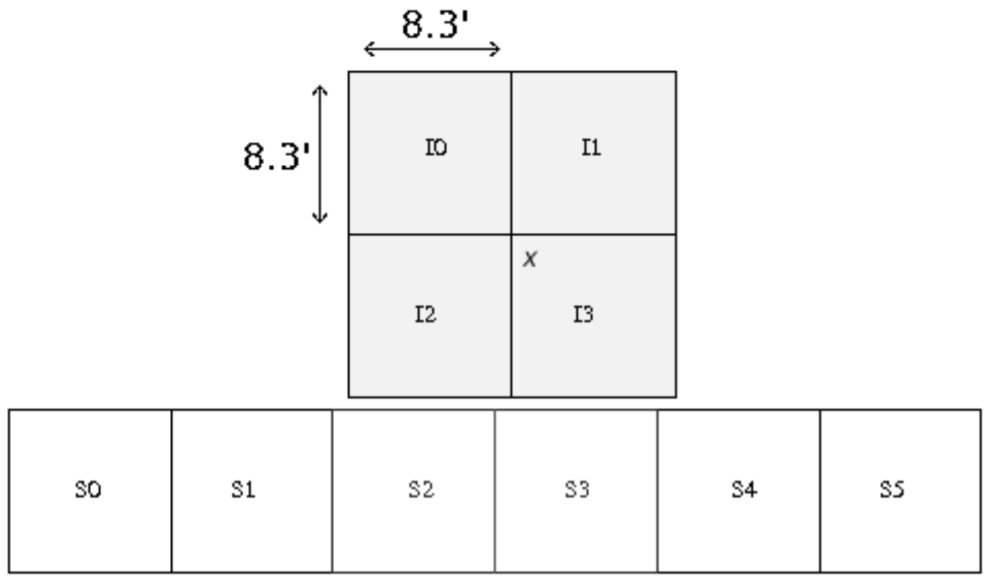
\includegraphics[scale=1]{images/chandra_acis_chips.png}}
\caption{Schematic of the Chandra's ACIS chips from \cite{weisskopf2002}. }
\label{imbeded_fb}
\end{figure}


Various configurations of ACIS are possible and each is better suited for different scientific uses. 
Using the labels used in Fig. 2.7, common configurations include the wide field imaging which uses all of ACIS-I (I0-I3) and the S2-S3 CCDs from ACIS-S.
This gives a field of view of $16.9' \times 16.9'$ plus $8.3' \times 16.9'$.
Another common configuration is the high resolution imaging which only uses the back illuminated S3 CCD without having to use any of the gratings. 
This provides a field of view of $8.3' \times 8.3'$.
In the 1-CCD chip mode, it is possible to subarray the chip to smaller dimensions. 
Typical subarrays restrict the CCD chip to 1/2, 1/4, or 1/8 of the original chip size in one dimension.
This reduces the field of view in that dimension to roughly 4', 2', or 1', respectively.
\citep{weisskopf2002}.

The other focal plane science instrument is the HRC, which is a microchannel plate (MCP) instrument also with two detectors: the HRC-I and the HRC-S. 
The HRC-I provides a field of view of $30' \times 30'$, the largest field of view of any Chandra detector. 
Thus, the HRI-I is used for wide-area imaging. The HRC-S is used for high resolution spectroscopy.

Lastly, Chandra has two transmission grating spectrometers, which are gold gratings that are placed behind the mirrors. 
The grating that is optimized for low energies  (0.07 - 0.2 keV) is called the Low Energy Transmission grating (LETG) and the other, which is optimized for higher energies ( 0.4-10 keV) is called the High Energy Transmission Grating (HETG).

\subsection{Chandra Souce Catalogs}

With the intent of providing a definitive catalog of the X-ray sources detected by Chandra, \cite{evans2010} constructed the Chandra Source Catalog (CSC).
The CSC was constructed largely using the ACIS-I, ACIS-S, and the HRC-I observations taken from the first eight years of Chandra’s mission. 
Recently, however, the second version of the CSC, called the CSC2.0, was officially released using similar but improved source detection methods as the CSC. 
This updated version included detections through the end of 2014 \citep{Evans2020}.

The CSC2.0 (just like CSC) was created using an automated data analysis and source detection pipeline.
The detection process started by using the observation IDs (image fields) to filter out observations that were conducted using the HRC-S, any grating observations, and any that included solar system and/or moving targets. 
This left most ACIS-I, ACIS-S, and HRC-I observations. 
Each one of these observations are then stacked with other observations that observed the same field of view, have a similar aimpoint (less than 1 arcmin so that the point spread function can be reliably combined), and were observed with the same instrument. 
For each stack, a pre-detection method picks out the brightest sources in each stack.
These sources are used in a “fine astrometry correction” step where the corrections needed to properly align the stacks are calculated. 
This results in having stacks that are aligned together up to less than a pixel and have more cohesive aspect solutions. 
For each observation in each stack, background flares candidates are removed from the observation to improve signal-to-noise ratio of the sources.
Full field background maps are then created and are used to simulate the counts necessary to detect a source.
The files are combined back into the stacks and combining with the background maps, an initial list of potential sources are created. 
A series of source-validation and maximum existence likelihood algorithms are used to verify the sources. 
Master match detections are created by stacking observations that overlap despite being from different instruments or having aimpoints separated by larger than 1 arcmin.
These are called the master sources and are given 2CXO catalog names. 
The CSC2.0 releases the detections found in each observation ID, in the stack observations, and in the master matches \citep{Evans2020}.

In total, the CSC2.0 includes information for 317,167 unique sources.
This was done using 928,280 individual observation detections from 10,382 ACIS and HRC-I images. 
This results in the source location map shown in Fig. 2.8. 
The false source rate is roughly 0.1 false source per field. 
The exposure times range from 0.6 ks to 5.9 Ms, with a median exposure of 12 ks.
There is a total sky coverage of 520 deg$^2$ in the B (Broad) band (0.5-7.0 keV) and 55 deg$^2$ for the W (Wide) band (0.1-10 keV) for the HRC \citep{Evans2020}.



\begin{figure}[H]
\centering
\scalebox{0.35}{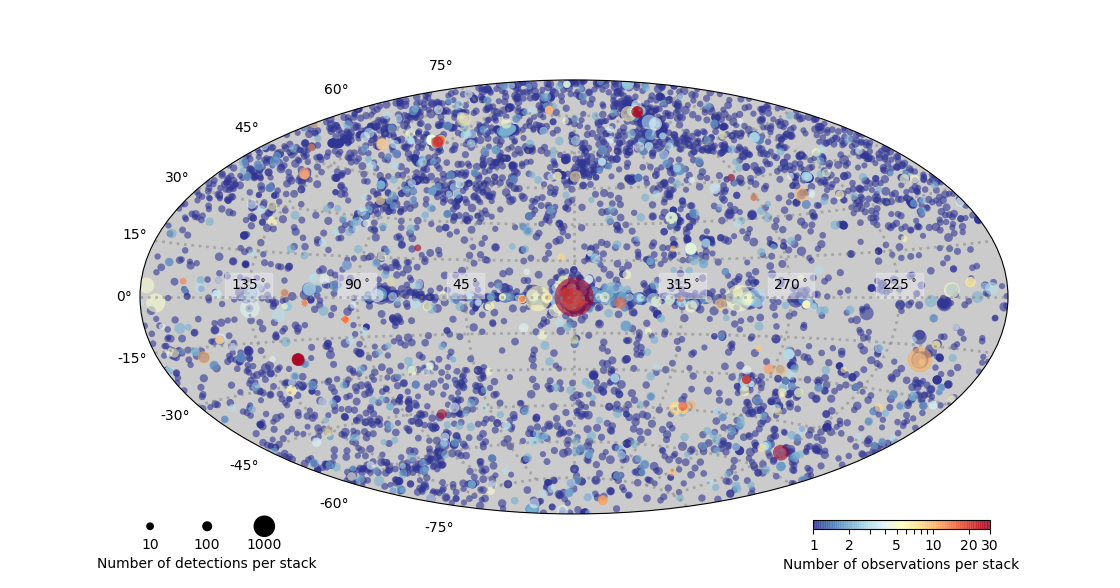
\includegraphics[scale=1]{images/csc2.png}}
\caption{Exposure map of the Chandra Source Catalog version 2.0 from \cite{Evans2020}. }
\label{imbeded_fb}
\end{figure}


\subsection{Optical Follow Up to Chandra Detections}

Since the CSC and CSC2.0 are relatively new and on-going catalogs that will likely be updated in future data releases, there are not many completed projects aimed at optically characterizing the sources in the catalog. 
However, efforts to characterize patches of sky observed by Chandra have been made for specific scientific goals. 
Of them, one of the larger projects (in terms of sky coverage) is the Chandra Multi-wavelength Project (ChaMP) survey \citep{kim2004} and the  Chandra Multiwavelength Plane (ChaMPlane) survey \citep{grindlay2005}.

The ChaMP survey cataloged serendipitous Chandra X-ray sources in a 14 deg$^2$ area.
The goal of the survey was to obtain samples of high redshift AGN and galaxy clusters \citep{kim2004}.
This catalog contained 486 X-ray sources. 
Optical follow up to these sources was conducted by \cite{green2004} where they found counterparts for 377 (78\%) of the sources. 
Obtaining spectra from observing runs, spectroscopic classifications were presented for 125 of them as well. Of these objects, 63, roughly 50\%, were broad line AGN and 28 were galaxies with narrow line emission \citep{green2004}.




%\section{Using the Catalogs}
%\label{2_4}

%We have chosen to work with the catalogs mentioned above: the Einstein 2sigma Catalog, the ROSAT all sky survey, and the CSC2.0. 
%This allows us to maximize the detection rate as we are maximizing the sources considered and the possibility that they are observed twice throughout the three catalogs. 
%Moreover, each of the catalogs do not overlap in their mission time and our baseline covers the 40 year history of X-ray astronomy, ideal conditions for studying long-term, dramatic X-ray variability.




